\documentclass[11pt,a4paper]{article}
\usepackage{a4wide}

\usepackage[english,dutch]{babel}
% better color management than parallel:
\usepackage{pdfcolparallel}

\setlength{\columnsep}{0.5cm}

%\usepackage{parallel}
\usepackage{color}
\usepackage{amsmath}
\usepackage{graphicx}

\usepackage{inconsolata} %a different monofont, texlive-fonts-extra needed!

\usepackage{arduinohighlight}


\usepackage{xcolor}
\usepackage{framed}
\colorlet{shadecolor}{gray!50}

\usepackage[
      %dvipdfm,    %put here the correct(!) driver you are using
      pdftex,
      unicode,
      colorlinks=true,    %no frame around URL
      urlcolor=blue,    %blue color
      menucolor=black,    %no colors
      linkcolor=blue,    %blue color
      bookmarks=true,    %tree-like TOC
      bookmarksopen=true,    %expanded when starting
      hyperfootnotes=false,    %no referencing of footnotes, does not compile
      pdfpagemode=UseOutlines,    %show the bookmarks when starting the pdf viewer
      pdfauthor={Ingegno.be},
      pdftitle={Line Follower - Ingegno.be},
]{hyperref}


\newtheorem{opdrE}{Task} 
\newenvironment{doE}
  {\begin{shaded}\begin{opdrE}}
  {\end{opdrE}\end{shaded}}

\newtheorem{opdrN}{Opdracht} 
\newenvironment{doN}
  {\begin{shaded}\begin{opdrN}}
  {\end{opdrN}\end{shaded}}
\newtheorem{code}{Code} 

%% First to \eng, then \ned, closes automatically with a paragraph
% \newcommand{\eng}[1]{\selectlanguage{english} \ParallelLText{#1}}
% \newcommand{\ned}[1]{\selectlanguage{dutch} \ParallelRText{#1} \ParallelPar}
% \newcommand{\engt}[1]{{#1} - }
% \newcommand{\nedt}[1]{{#1}}
% \newcommand{\engo}[1]{\eng {#1}}
% \newcommand{\nedo}[1]{\ned {#1}}

%% Use following for book in English language
% \usepackage{multicol}
% %\newcommand{\eng}[1]{\selectlanguage{english} {#1}}
% \newcommand{\eng}[1]{\begin{multicols}{2}{\selectlanguage{english} {#1}}\end{multicols} \hrule}
% \newcommand{\ned}[1]{ }
% \newcommand{\engt}[1]{{#1}}
% \newcommand{\nedt}[1]{ }
% \newcommand{\nedo}[1]{ }
% \newcommand{\engo}[1]{\selectlanguage{english} {#1}}

%% Use following for book in Dutch language
\usepackage{multicol}
%\newcommand{\ned}[1]{\selectlanguage{dutch} {#1}}
\newcommand{\ned}[1]{\begin{multicols}{2}{\selectlanguage{dutch} {#1}}\end{multicols} \hrule}
\newcommand{\eng}[1]{ }
\newcommand{\nedt}[1]{{#1}}
\newcommand{\engt}[1]{ }
\newcommand{\engo}[1]{ }
\newcommand{\nedo}[1]{\selectlanguage{dutch} {#1}}


%\selectlanguage{english}
% \ParallelLText{\blindtext}
%\selectlanguage{dutch}
%\ParallelRText{\blindtext}
%\ParallelPar


\begin{document}


 \title{Lijnvolger robot!}
 \author{Ingegno Team: M.C. Ciocci, B. Malengier}
 \date{\today}
 \maketitle

\begin{figure}[h]
  \centering
  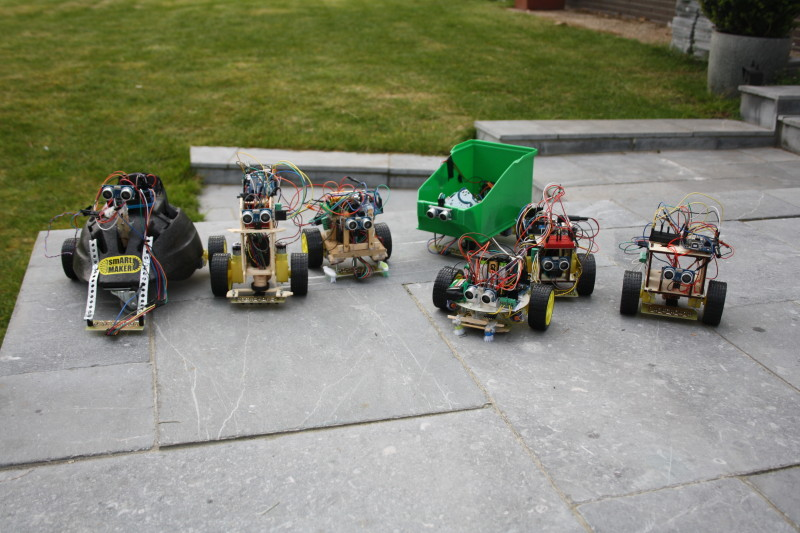
\includegraphics[width=9cm]{pic/robotteam.jpg}
%\caption{\engt{Ingegno line following robots}
%\nedt{Ingegno lijnvolg robots}}
\label{f:ingrobots}       % Give a unique label
\end{figure}

\begin{Parallel}{7.5cm}{7.5cm}

\section{\engt{Introduction} \nedt{Introductie}}
\eng{TODO
}

\ned{We maken een lijnvolg robot. Dit is een ingewikkeld project, met veel programmatie
}

\subsection{\engt{The components} \nedt{De componenten}}
\eng{We will need the following components: 
\begin{enumerate}
 \item TODO
\end{enumerate}
You will also need a soldering iron, and optionally you can make a cover for the cube, eg using 3D printing.

For an overview of meaning of the components, see the cheat sheet distributed seperately.
}

\ned{We zullen volgende componenten gebruiken: 
\begin{enumerate}
 \item TODO
\end{enumerate}
Je zal ook een soldeerijzer nodig hebben.

Voor een overzicht van de betekenis van de componenten, zie het overzicht die je apart gekregen hebt.
}

\subsection{Arduino}
\eng{We will make intensive use of Arduino, so you need to install the \href{http://Arduino.cc}{Arduino software}. Once installed, you can connect the Arduino to your PC via de \textsc{usb} port.  In the programming environment you installed you can write programs, and load those on the Arduino board. They will be executed there as long as the Arduino has power.

}
\ned{We zullen intensief gebruik maken van Arduino, dus moet je de \href{http://Arduino.cc}{Arduino software} installeren op je laptop.
Eenmaal geinstalleerd kun je nu je Arduino koppelen aan je computer via de \textsc{usb} poort. In de programmeeromgeving van Arduino kun je programma's schrijven en die opladen naar de Arduino, waar ze dan uitgevoerd worden zolang er stroom is.
}


\subsection{\engt{Programming with Arduino} \nedt{Programmeren met Arduino}}
\eng{A programming language needs to be understood by a computer. Unfortunately computers are still a little bit dumb, so you are not allowed to make errors! It's like a writing contest in which you need to obtain a 10/10 every time. So take time to learn the form of the language. See the specific sheet 'Programming with Arduino' distributed with this manual.}


\ned{Een programmeertaal moet verstaan worden door een computer. Spijtig genoeg zijn computers nog altijd een beetje dom, dus mag je geen enkele fout maken! Het is zoals een dictee waar je altijd 10/10 moet halen. Neem dus de tijd om de structuur en taal van de Arduino te leren. Zie de blaadjes 'Programmeren met Arduino' die je bij deze gids kan downloaden.}

\section{\engt{Lesson 1: Drive!} \nedt{Les 1: Rijden maar}}
\eng{TODO}.
\ned{We beginnen met de motoren monteren en uittesten. }

\begin{code}\label{c:l1_motor}
 \ \newline
\inputardfull{\string"../sketches/calib_motors_forward/calib_motors_forward.ino\string"}
\end{code}

\section{\engt{Lesson 2: Light sensor setup} \nedt{Les 2: een lichtsensor gebruiken}}
\eng{TODO}.
\ned{De tweede stap is het monteren van de lichtsensor. De lichtsensor kan kleuren detecteren onder de sensor.}


\begin{code}\label{c:l2_c}
 \ \newline
\inputardfull{\string"../sketches/calib_light_sensor_setpoint_line_follow/calib_light_sensor_setpoint_line_follow.ino\string"}
\end{code}


\section{\engt{Lesson 3: Follow a line} \nedt{Les 3: Een lijn volgen}}
\eng{TODO}.
\ned{Met motoren en de lichtsensor kunnen we een lijn volgen
}

\subsection{\engt{Basic version: move to midline} \nedt{Basisversie: beweeg naar een middellijn}}

\eng{TODO}
\ned{Ons basisalgoritme werkt op basis van volgend principe: 
\begin{enumerate}
 \item We lezen de lichtsensor in. We bepalen het middelpunt zoals in les 2: gewogen gemiddelde van de 5 sensoren. Gezien deze van 0 tot en met 4 lopen, zou het midden 2 moeten zijn. 
 \item De fout is het verschil van het gemeten middelpunt en het gewenste middelpunt, maal 1000. We willen deze fout zo klein mogelijk houden.
 \item Op basis van de fout passen we de snelheid van de motoren aan in de functie \ardo{calc\_turn}. De snelheid van de motoren is een getal tussen \ardo{min\_speed} en \ardo{max\_speed}, waarbij de eerste de waarde van PWM is die overeenkomt met stilstand (typisch 0), en \ardo{max\_speed} de maximum snelheid die je wil (typisch 180 tot 254). We corrigeren de snelheid van de linker of rechtermotor dus met
$$\frac{\mathrm{fout}}{\mathrm{max\_fout}} \times ( \mathrm{max\_speed} - \mathrm{min\_speed} ).
$$
 \item De correctie wordt verminderd van de snelheid van het wiel dat rotatie in de correcte richting veroorzaakt.
\end{enumerate}
}

\begin{code}\label{c:l3_c}
 \ \newline
\inputardfull{\string"../sketches/calib_forward_line_follow/calib_forward_line_follow.ino\string"}
\end{code}

\subsection{\engt{Extended version: types of lines} \nedt{Uitgebreide versie: type lijnen}}

\eng{TODO}
\ned{Ons basisalgoritme werkt op eenvoudige, traag draaiende lijnen. Zodra het wat sneller gaat, of bij scherpe bochten gaat het mis. Er kunnen verschillende manieren bedacht worden om dit op te lossen. 

Laat ons de volgende aanpak kiezen: we bepalen een type lijn. In plaats van enkel in \ardo{sensors_read()} te bepalen of we een lijn zien of niet, onderscheiden we volgende gevallen, die we als geheel getal (integer, dus int) teruggeven:
\begin{enumerate}
 \item \ardo{#define LS\_UNKNOWN    0 // we kunnen niet bepalen wat we zien}
 \item \ardo{#define LS\_BLACKLINE  1 // een zwarte lijn}
 \item \ardo{#define LS\_BLACKFIELD 2 // een zwart veld}
 \item \ardo{#define LS\_WHITEFIELD 3 // een wit veld}
 \item \ardo{#define LS\_BLACKLEFT  4 // zwart afbuigend naar rechts}
 \item \ardo{#define LS\_BLACKRIGHT 5 // zwart afbuigend naar links}
 \item \ardo{#define LS\_BLACKSPLIT 6 // zwart links en rechts, niet midden}
\end{enumerate}
Pas de functie \ardo{sensors_read()} aan om op basis van de gemeten waarden te bepalen wat er gebeurt. Pas dan de \ardo{loop()} functie aan met een switch op basis van het resultaat: \ardo{switch (sensors_read())}. Voor \ardo{LS\_BLACKLINE} is het zoals in de basisversie, maar doe nu andere bewegingen in de andere gevallen.

Onze aanpak kun je vinden op \url{https://github.com/ingegno/linefollower1/blob/master/sketches/calib_forward_line_follow_extend/calib_forward_line_follow_extend.ino}.
}

\section{\engt{Lesson 4: Distance to an object} \nedt{Les 4: Afstand tot een object.}}
\eng{TODO}

\ned{We plaatsen nu ogen op onze robot. De ogen zijn in werkelijkheid ultrasone sensoren, die de afstand bepalen tot objecten voor zich op dezelfde wijze als vleermuizen dat doen. 

De code kan gevonden worden in \ref{c:l4_c}.
}

\begin{code}\label{c:l4_c}
 \ \newline
\inputardfull{\string"../sketches/calib_distance_sensor/calib_distance_sensor.ino\string"}
\end{code}



\section{\engt{Lesson 5: Search and push object} \nedt{Les 5: Zoek en duw object.}}
\eng{TODO}

\ned{Integreer nu de code uit les 4 in de code van les 3. Zorg dat de robot niet rijdt als niet op een zwarte lijn. We zullen nu het volgende probleem beschouwen: Veronderstel dat je op een zwarte lijn was, en op een wit veld komt. Verifieer of dat waar is (dus je echt op een zwarte lijn was). Zoek op het witte veld een object, en duw het uit het veld.

In de code zullwen we dus in het geval van \ardo{case LS\_WHITEFIELD:}, code uitvoeren om dit te bereiken. Gezien onze code in de loop de lijn probeert te lezen, en we nu iets anders moeten doen dat vastligt (zoeken, bewegen naar, en dan wegduwen), doen we alles zonder gebruik te maken van de Arduino loop. Met andere woorden, we gebruiken de \ardo{while (allesok)} constructie om acties te laten voortduren tot we een gewenst resultaat hebben.

De veranderingen kunnen gevonden worden in \ref{c:l5_c}.
}

\begin{code}\label{c:l5_c}
 \ \newline
\inputard{\string"../sketches/calib_search_push_object/calib_search_push_object.ino\string"}{59}{75}
 \ \newline
\inputard{\string"../sketches/calib_search_push_object/calib_search_push_object.ino\string"}{163}{321}
\end{code}


\end{Parallel}
\end{document}